\documentclass[aspectratio=169,10pt]{beamer}
% Clean default theme (metropolis not installed)
\usetheme{default}
\usecolortheme{seahorse}
\usefonttheme{professionalfonts}
\setbeamertemplate{navigation symbols}{}
\setbeamertemplate{footline}[frame number]
\setbeamercolor{frametitle}{fg=white,bg=structure!80!black}
\setbeamertemplate{frametitle}{\vskip4pt\usebeamerfont{frametitle}\insertframetitle\par}
\setbeamercolor{block title}{bg=structure!20!white,fg=black}
\setbeamerfont{frametitle}{size=\large,series=\bfseries}

\usepackage{graphicx}
\usepackage{booktabs}
\usepackage{xcolor}
\usepackage[skins]{tcolorbox}
\graphicspath{{../figures/}}
\newcommand{\best}[1]{{\color{green!45!black}\textbf{#1}}}
\newcommand{\bad}[1]{{\color{red!60!black}#1}}
% key-message strip at the bottom of a frame, kept clear of figures
\newcommand{\takeaway}[1]{\vfill\begin{tcolorbox}[colback=structure!12!white,colframe=structure!60!black,
  boxrule=0.4pt,left=4pt,right=4pt,top=2pt,bottom=2pt]\small #1\end{tcolorbox}}

\title{\bfseries Grouping Enzymatic Reactions by EC Number}
\subtitle{Benchmarking reaction embeddings \& clustering, and a fusion method that beats them}
\author{ModelSEED reaction--representation study}
\date{\today}

\begin{document}

{\setbeamertemplate{footline}{}
\begin{frame}[plain]
  \titlepage
  \begin{center}\small 13{,}721 reactions $\cdot$ 21 embeddings $\times$ 12 clustering algorithms $\cdot$ EC-purity + retrieval\end{center}
\end{frame}}

% ---------------------------------------------------------------
\begin{frame}{The question}
  \begin{columns}[T]
    \begin{column}{0.58\textwidth}
      \textbf{Goal.} Given ModelSEED reactions, find the (reaction embedding,
      clustering algorithm) combination that groups reactions so each cluster is
      \emph{clean} with respect to its \textbf{EC number} --- reactions of the same
      enzyme class together, different classes apart.

      \vspace{6pt}
      \textbf{Why it matters}
      \begin{itemize}\small
        \item EC \textbf{annotation transfer} to unlabelled reactions
        \item \textbf{Curation}: flag EC mis-assignments (outliers in a clean cluster)
        \item A reaction \textbf{similarity index} (FAISS) for metabolic modelling
      \end{itemize}
    \end{column}
    \begin{column}{0.40\textwidth}
      \begin{block}{Dataset}\small
        \begin{tabular}{@{}ll@{}}
          reactions & 13{,}721\\
          full EC (4-level) & 5{,}622\\
          EC3 subclasses & 261\\
          EC2 / EC1 & 68 / 7\\
        \end{tabular}\\[3pt]
        non-obsolete, full EC, all compounds have SMILES.
      \end{block}
      \footnotesize Primary metric: \textbf{EC3 AMI} (chance- \& count-corrected).
      Also EC1/EC2/full, homogeneity, purity, and kNN retrieval.
    \end{column}
  \end{columns}
\end{frame}

% ---------------------------------------------------------------
\begin{frame}{What we surveyed}
  \begin{columns}[T]
    \begin{column}{0.33\textwidth}
      \begin{block}{Embeddings (21)}\footnotesize
        \textbf{Structural (diff):} ECFP2/4/6, AtomPair, RDKit, MACCS, MHFP, DRFP, Avalon, torsion\\[2pt]
        \textbf{PhysChem:} 217 physicochemical descriptors\\[2pt]
        \textbf{Learned:} RXNFP, ChemBERTa, MolFormer\\[2pt]
        \textbf{Atom-mapped:} CGR (linear/morgan)
      \end{block}
    \end{column}
    \begin{column}{0.33\textwidth}
      \begin{block}{Clustering (12)}\footnotesize
        K-means, Agglomerative (avg/complete/single/Ward), Birch,
        \textbf{Leiden}, \textbf{Louvain}, Spectral, DBSCAN, HDBSCAN, Butina
      \end{block}
    \end{column}
    \begin{column}{0.33\textwidth}
      \begin{block}{Evaluation}\footnotesize
        Common 256-d SVD / cosine space.\\[2pt]
        \textbf{Clustering:} AMI, homogeneity, V-measure, purity at EC1/2/3/full.\\[2pt]
        \textbf{Retrieval:} leave-one-out kNN EC accuracy.
      \end{block}
    \end{column}
  \end{columns}
  \takeaway{One harness, every embedding $\times$ every algorithm, scored identically --- 550+ configurations.}
\end{frame}

% ---------------------------------------------------------------
\begin{frame}{Result 1 --- the benchmark grid}
  \centering
  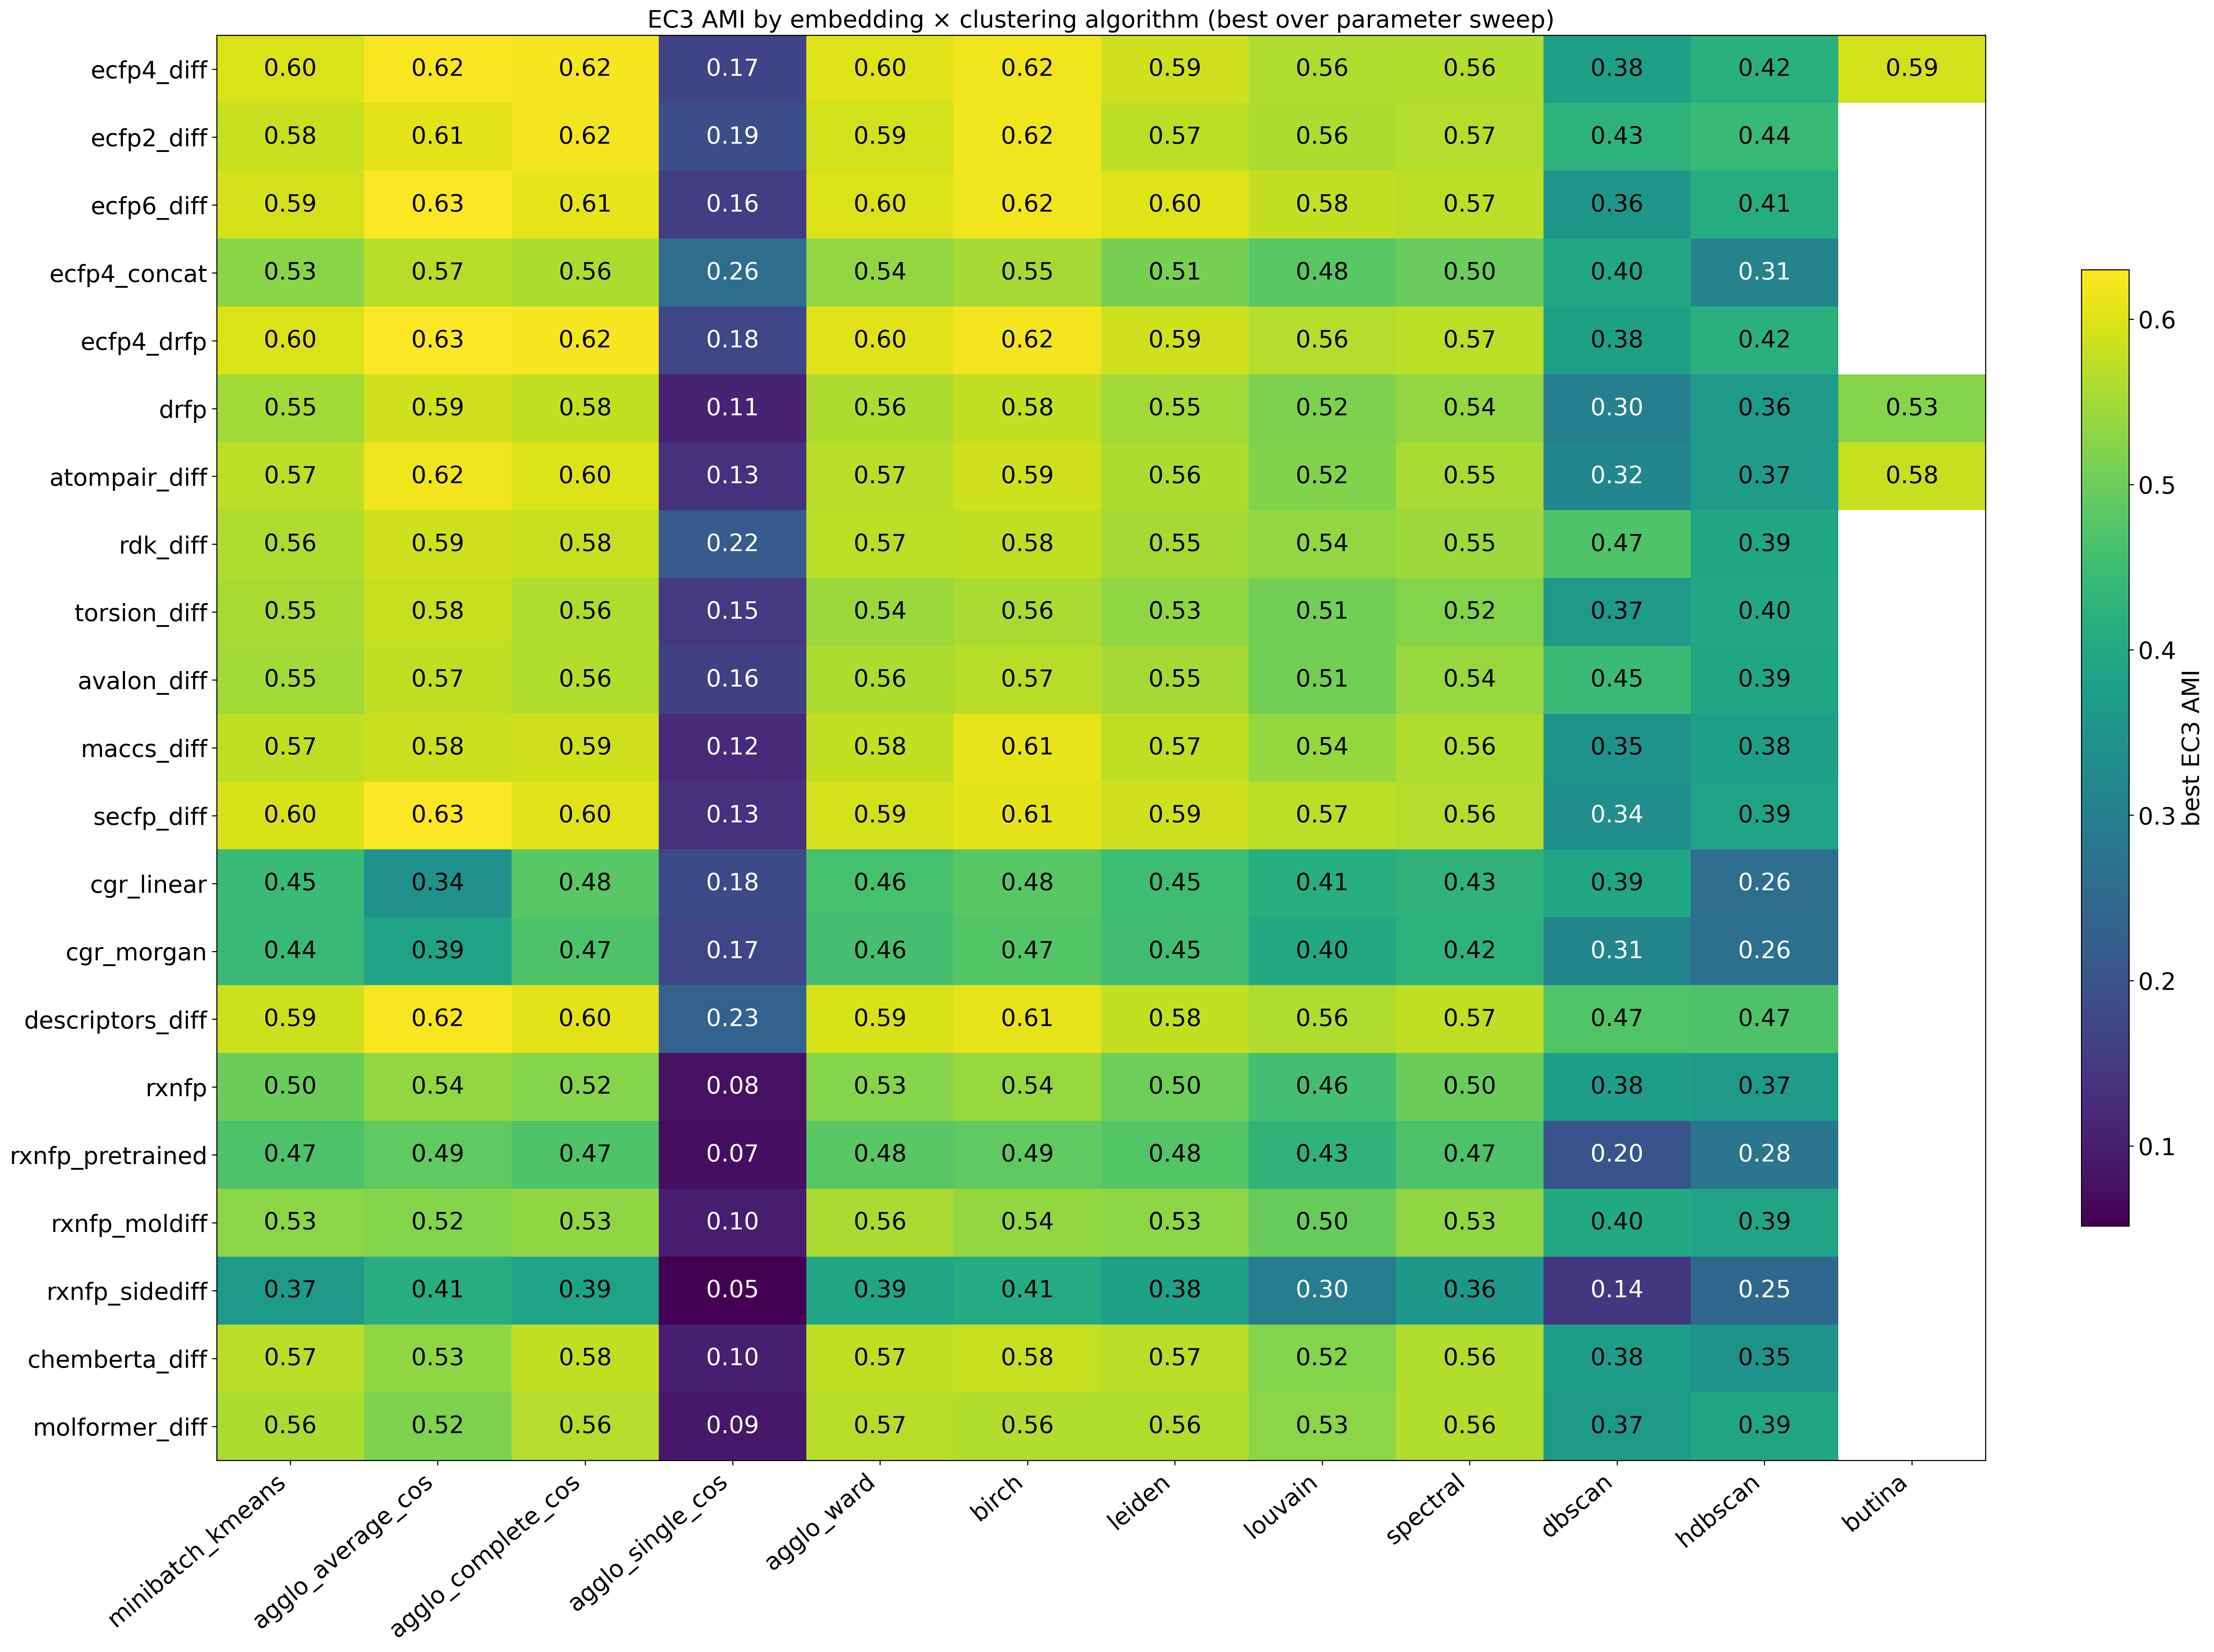
\includegraphics[height=0.80\textheight]{fig_heatmap_embed_algo.png}\\[-1pt]
  {\scriptsize CGR rows are full-set (coverage-limited to 75\%); the fair CGR comparison is on a later slide.}
\end{frame}

\begin{frame}{Result 1 --- what wins}
  \begin{columns}[T]
    \begin{column}{0.5\textwidth}
      \centering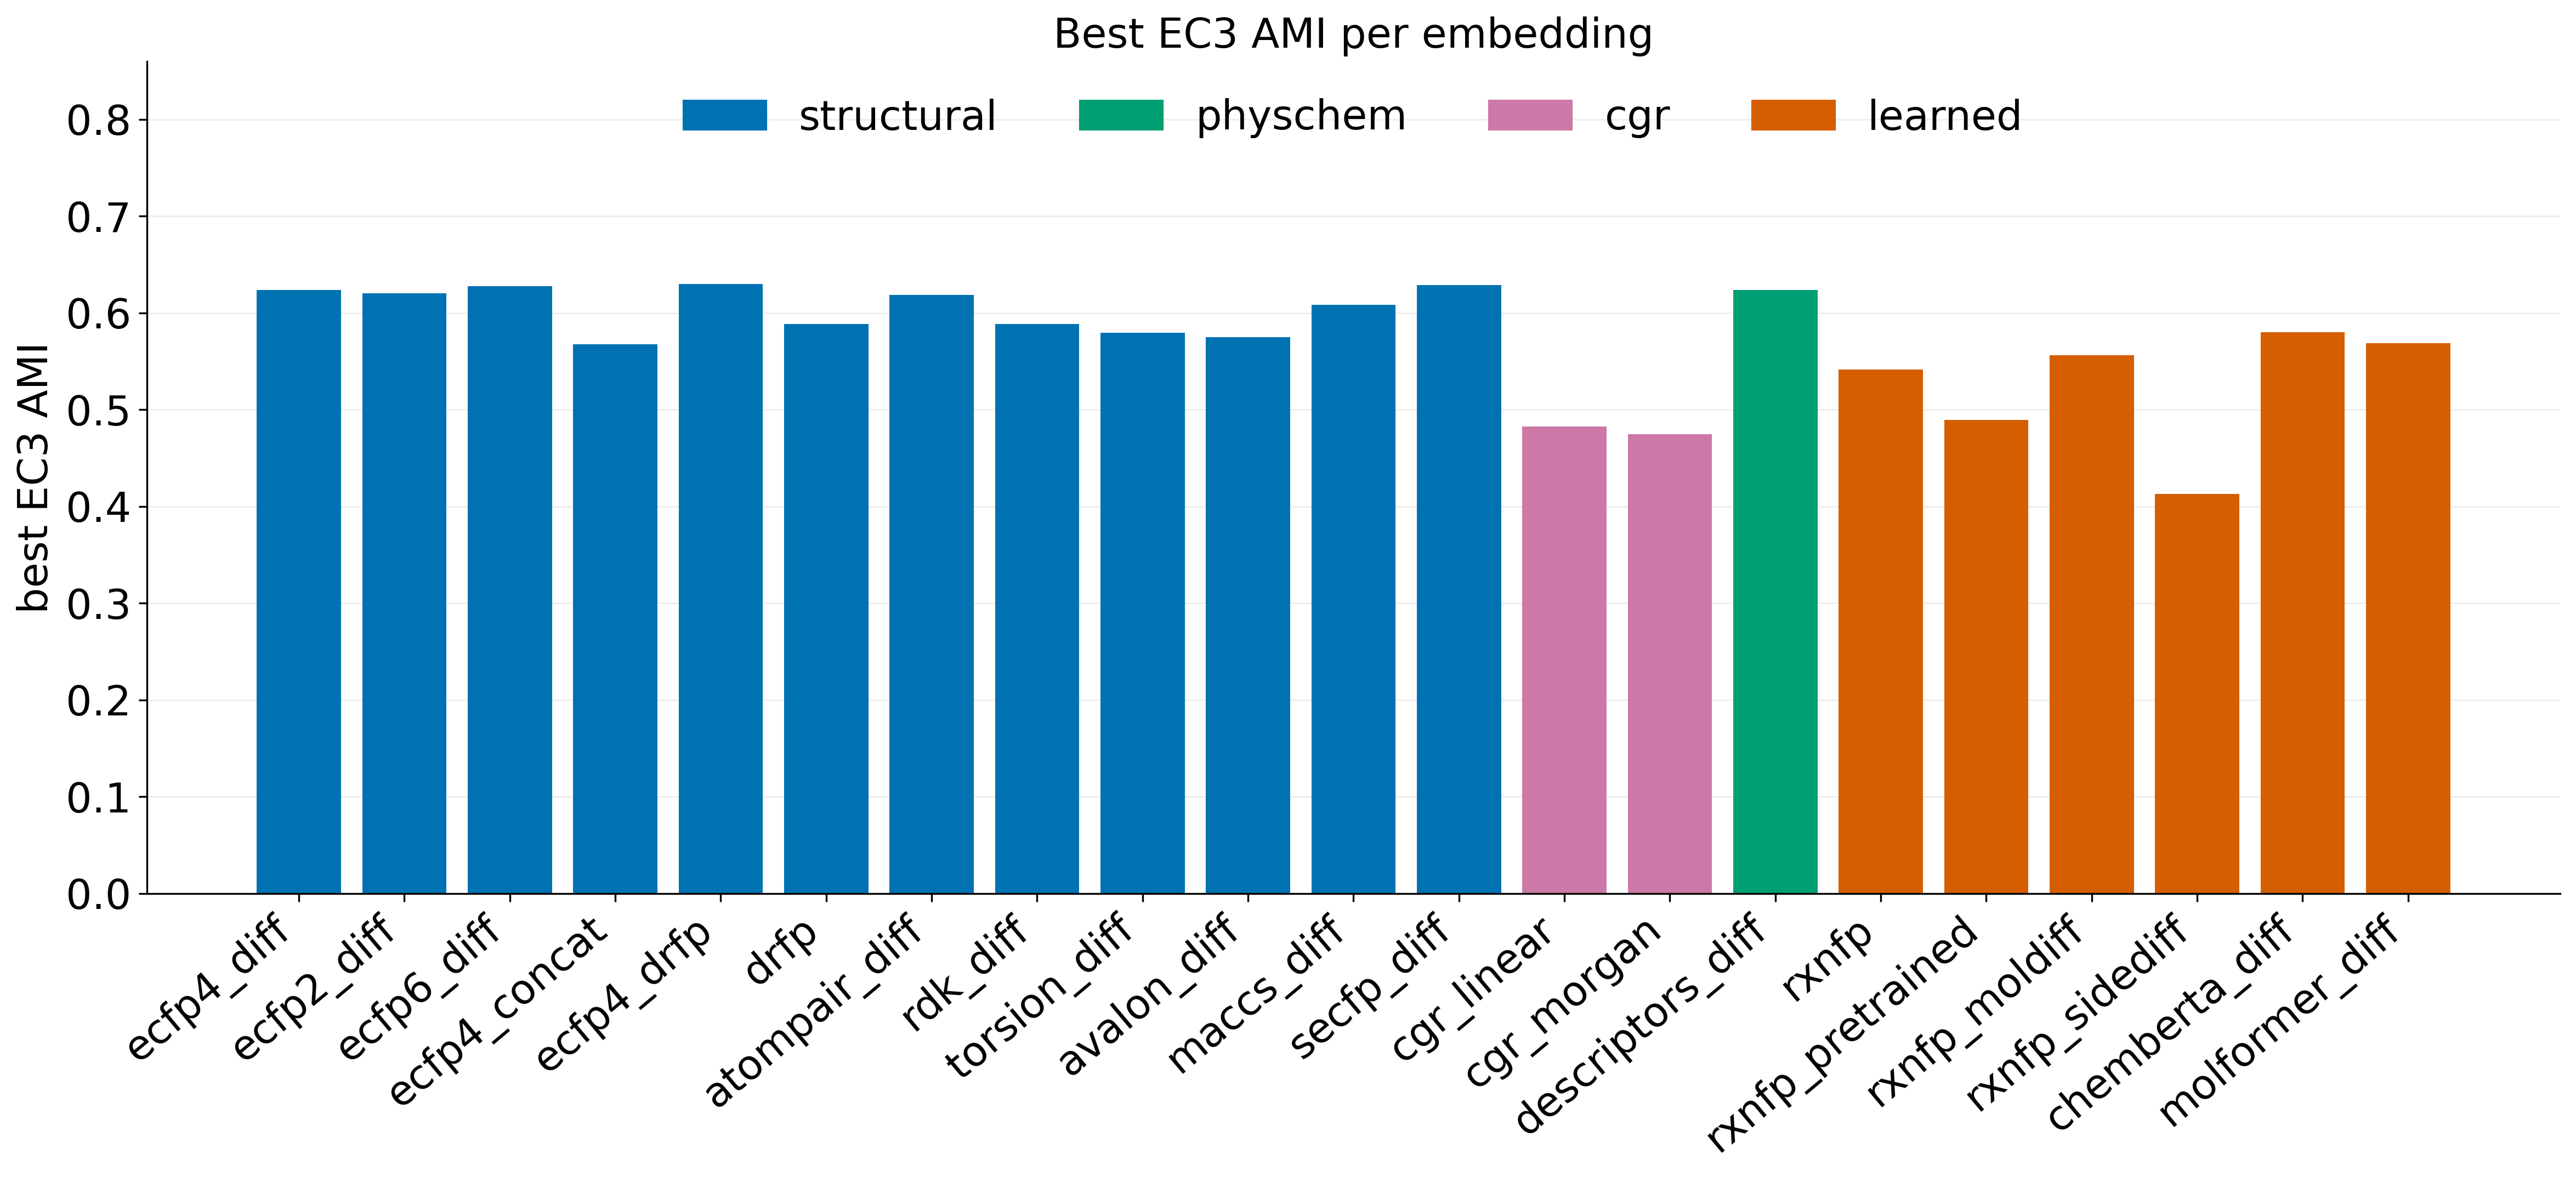
\includegraphics[width=\linewidth]{fig_best_per_embedding.png}
    \end{column}
    \begin{column}{0.5\textwidth}\small
      \begin{itemize}
        \item Structural \emph{difference} fingerprints form a \best{plateau} at EC3 AMI $\approx$0.62--0.63 --- radius/type barely matter.
        \item \best{PhysChem} (217 physicochemical descriptors) are a surprise: highest homogeneity/purity.
        \item \best{Agglomerative average/complete} + Birch win; \bad{single-linkage collapses}; density (DBSCAN/HDBSCAN) weakest.
        \item \bad{Learned embeddings underperform} (RXNFP worst).
      \end{itemize}
    \end{column}
  \end{columns}
\end{frame}

% ---------------------------------------------------------------
\begin{frame}{Result 2 --- retrieval $\gg$ clustering}
  \begin{columns}[T]
    \begin{column}{0.56\textwidth}
      \centering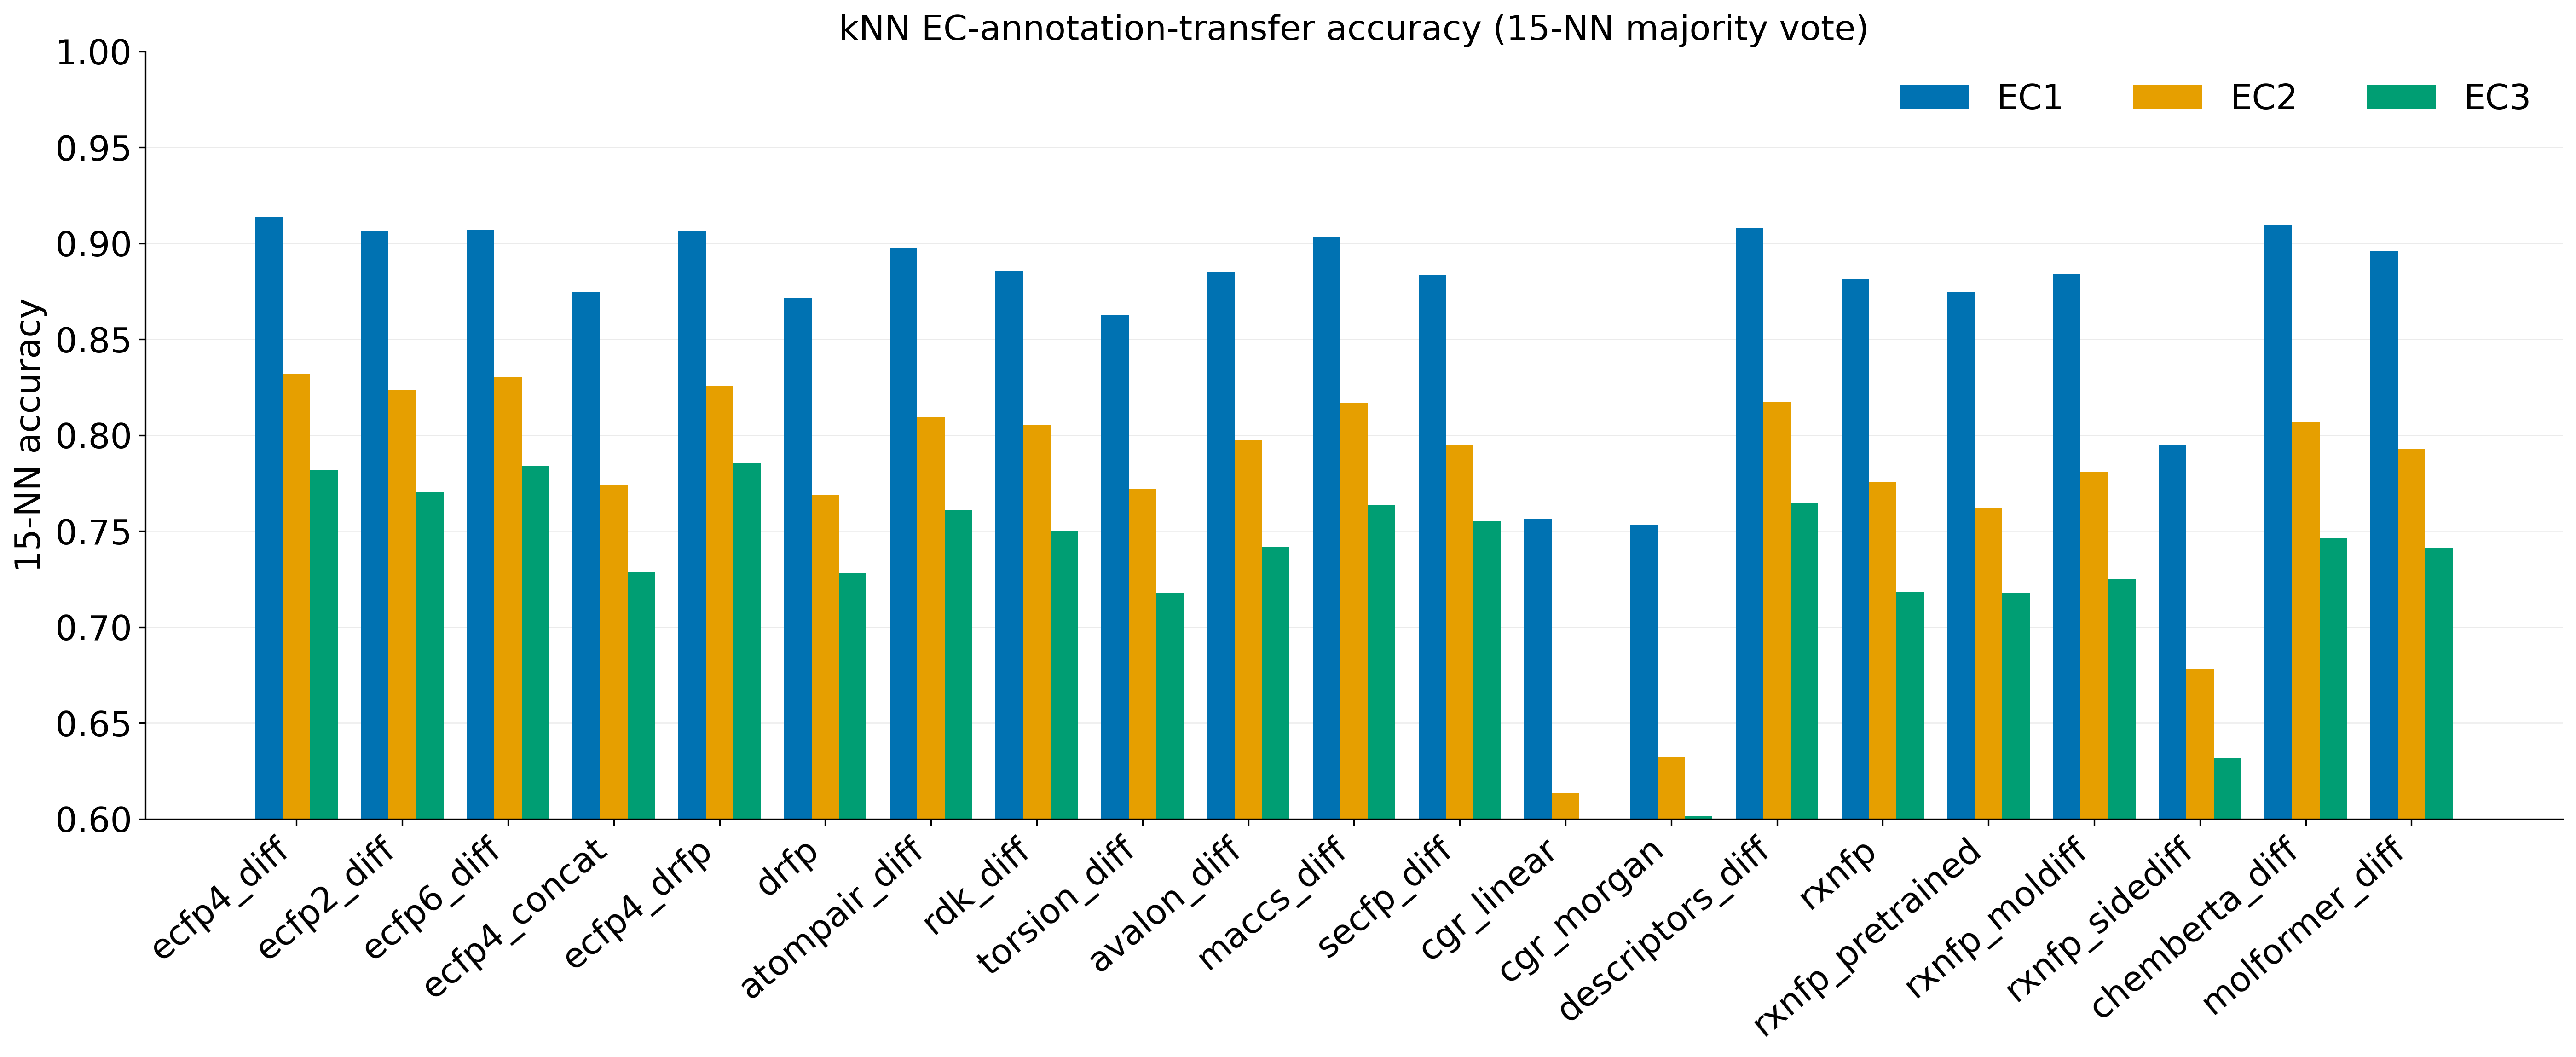
\includegraphics[width=\linewidth]{fig_knn_transfer.png}
    \end{column}
    \begin{column}{0.44\textwidth}\small
      Cluster AMI tops out near 0.63, but \textbf{nearest-neighbour retrieval} is far stronger:
      \begin{itemize}
        \item 15-NN: EC1 \best{0.91}, EC2 0.83, EC3 0.78
        \item confidence-gated: \best{EC3 0.90 accuracy over 76\%} of reactions
      \end{itemize}
      \textbf{Reading:} the representation already knows EC \emph{locally}; unsupervised
      partitioning loses it \emph{globally}. This is the biggest untapped lever.
    \end{column}
  \end{columns}
  \takeaway{For annotation, don't cluster --- \textbf{retrieve}. Full 4-level EC stays hard everywhere ($\sim$0.3--0.5).}
\end{frame}

% ---------------------------------------------------------------
\begin{frame}{The reaction map}
  \centering
  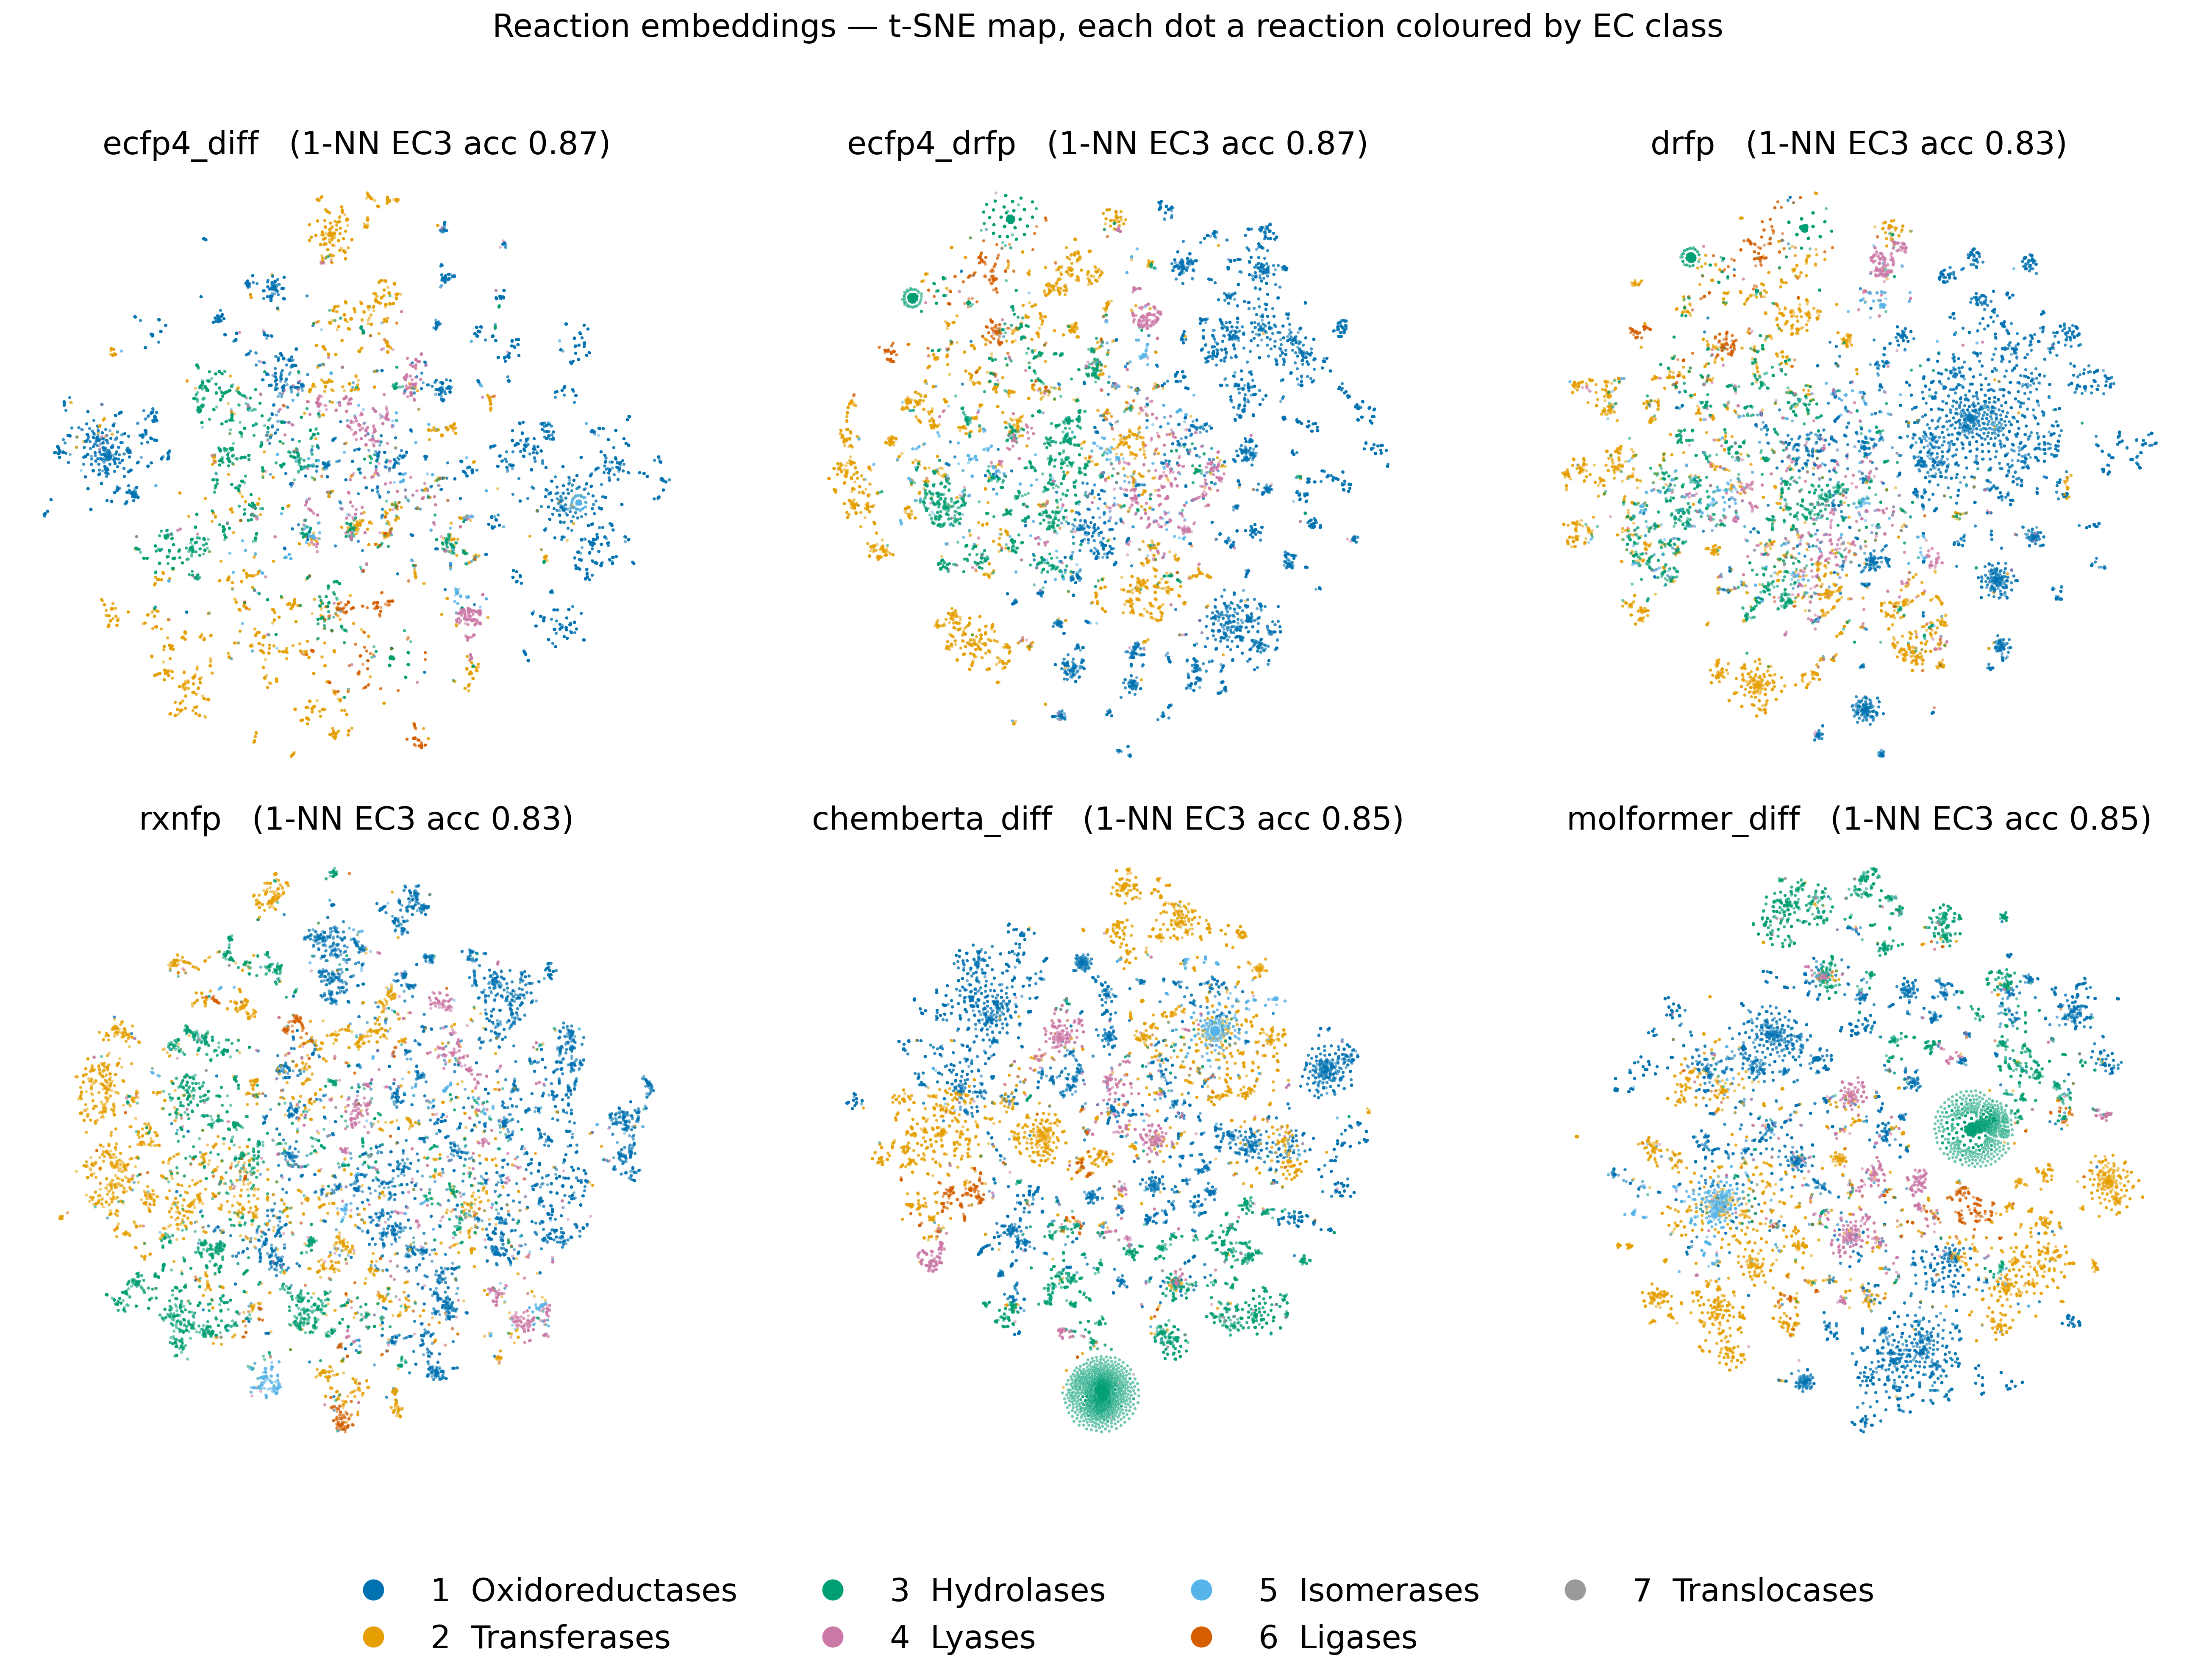
\includegraphics[height=0.80\textheight]{fig_tsne_ec_comparison.png}
\end{frame}

% ---------------------------------------------------------------
\begin{frame}{Why does RXNFP underperform?}
  \begin{columns}[T]
    \begin{column}{0.54\textwidth}
      \centering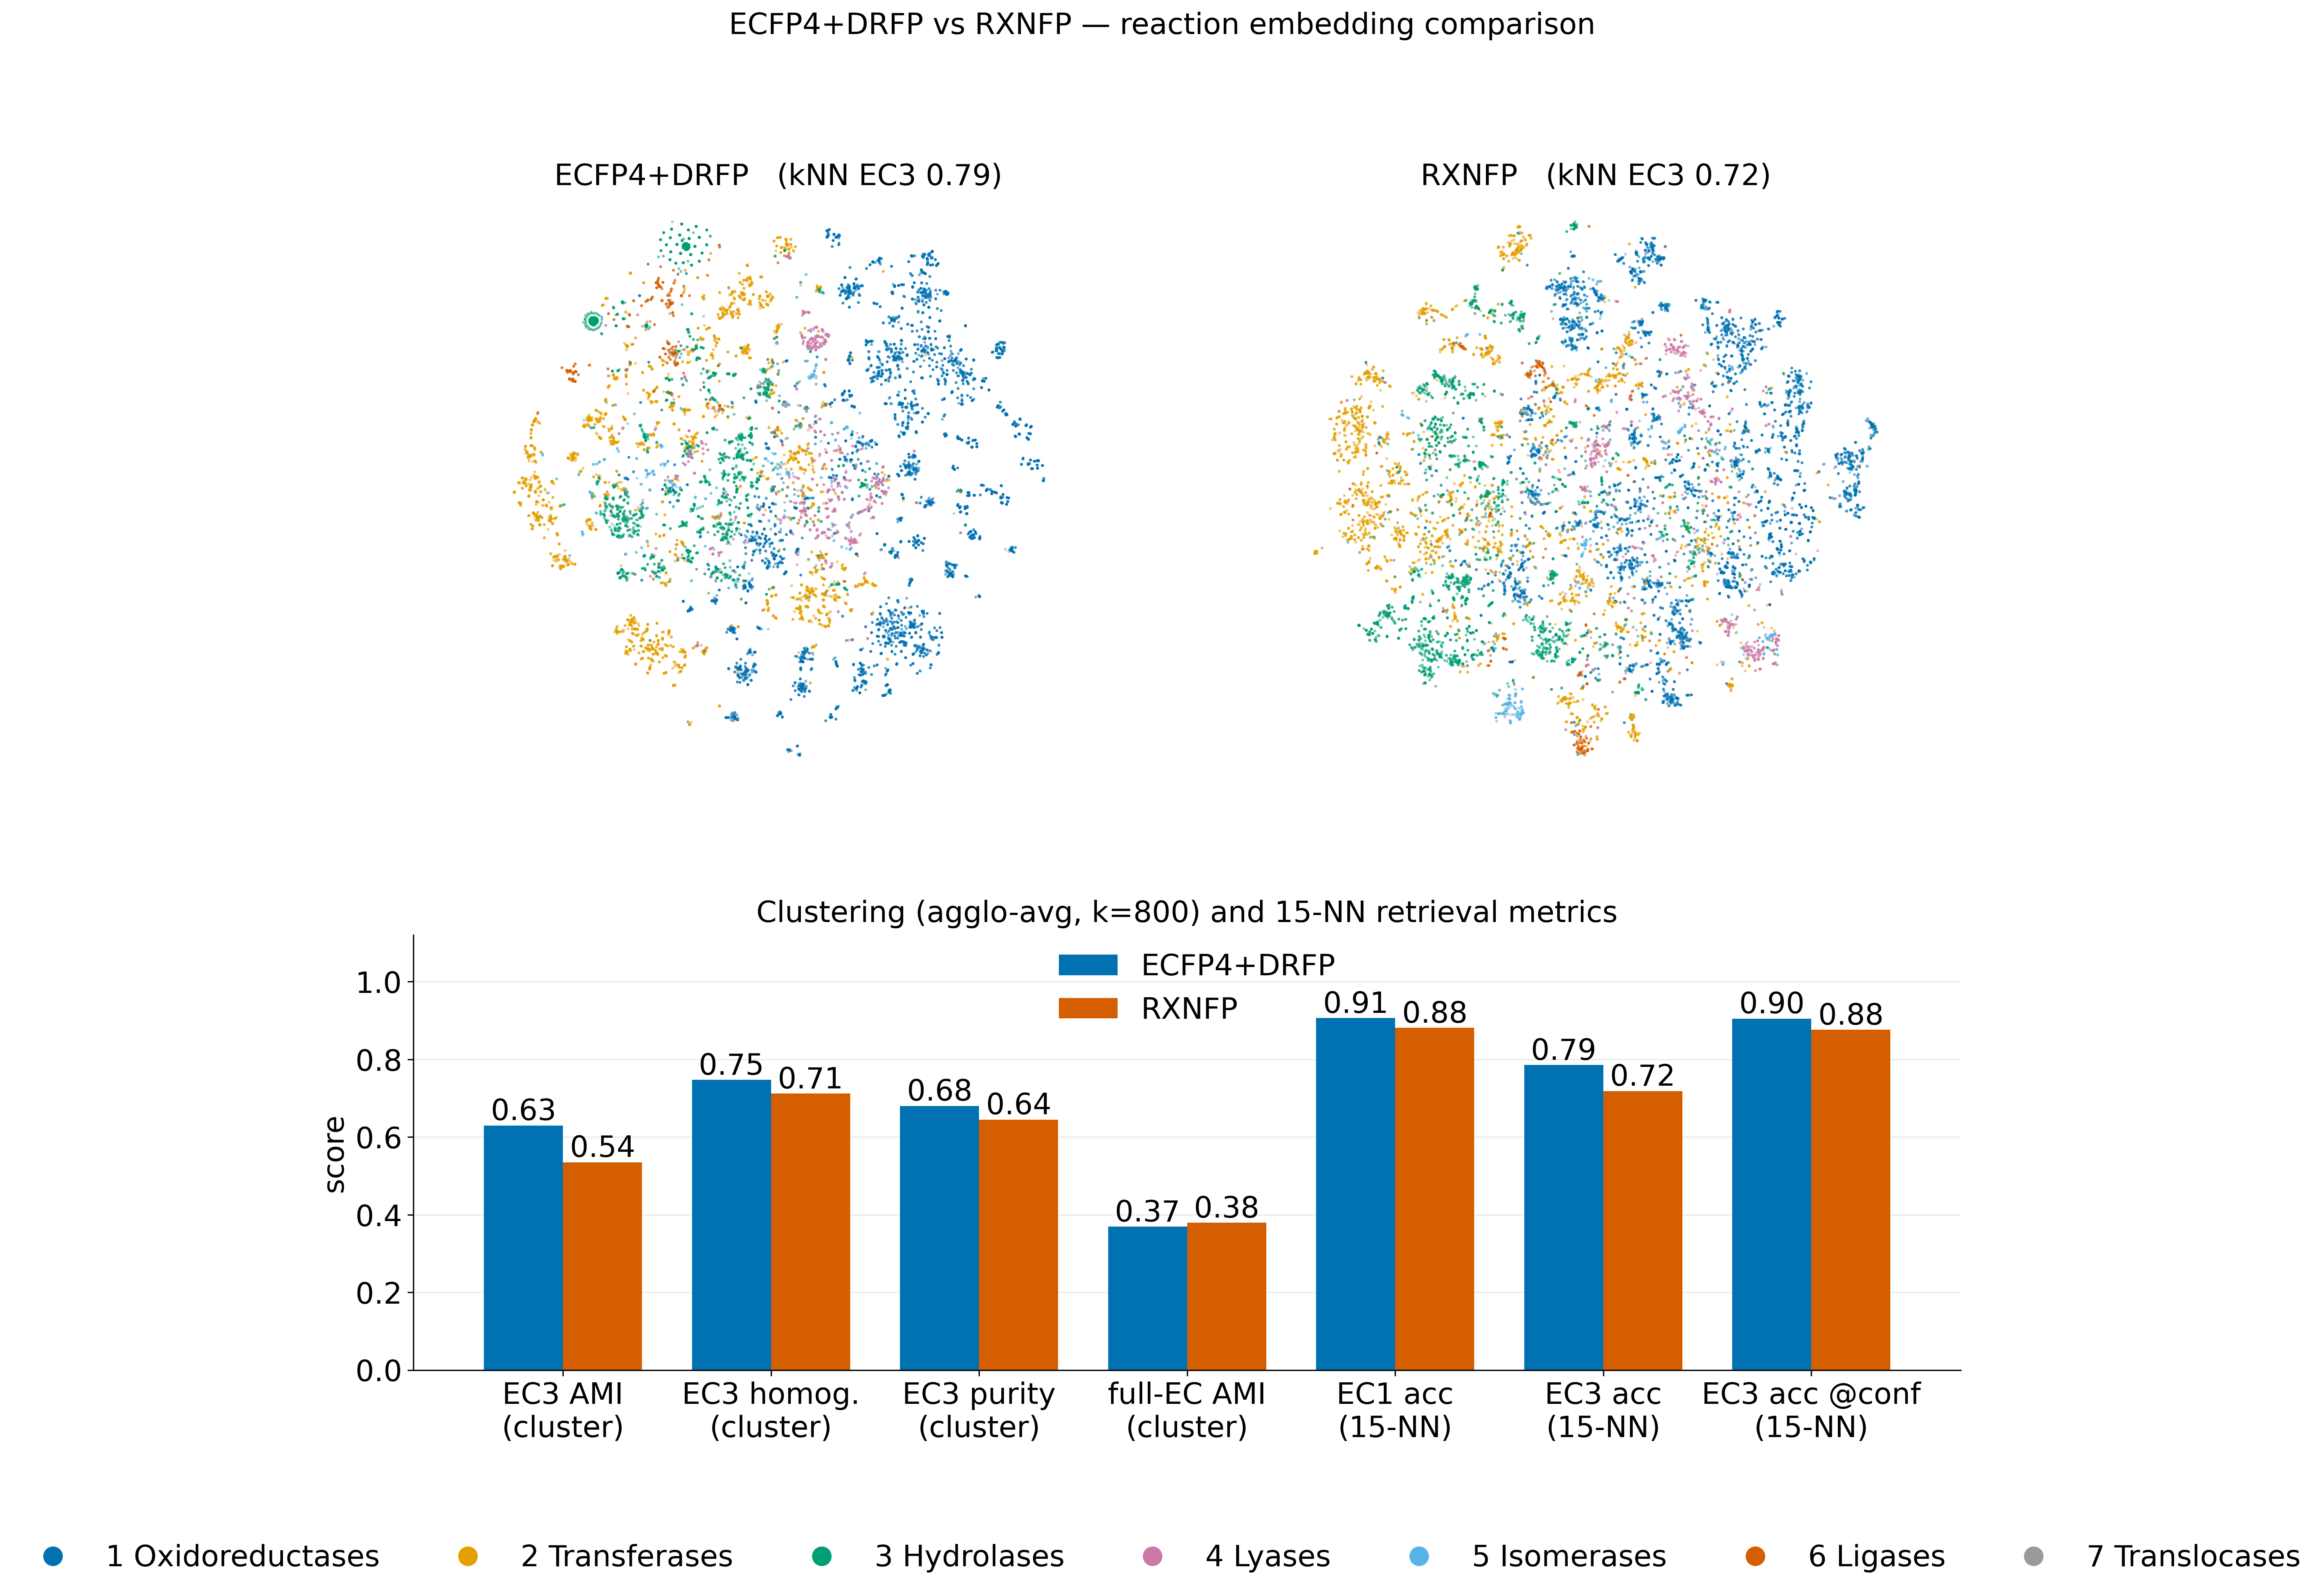
\includegraphics[width=\linewidth]{fig_compare_ecfp4drfp_vs_rxnfp.png}
    \end{column}
    \begin{column}{0.46\textwidth}\small
      RXNFP (pretrained rxn-BERT) trails a cheap fingerprint on every EC metric.
      \begin{itemize}
        \item \textbf{Distribution:} trained on USPTO \emph{organic synthesis}, not enzymatic biochemistry.
        \item \textbf{Taxonomy:} fine-tuned for organic reaction-type classes, not EC.
        \item \textbf{No difference operation:} a holistic latent; cofactors dominate.
      \end{itemize}
      We tested adding a difference (\texttt{rxnfp\_moldiff}): only a hair better ---
      confirming the ceiling is \emph{training}, not the difference construction.
    \end{column}
  \end{columns}
\end{frame}

% ---------------------------------------------------------------
\begin{frame}{Attacking full-EC: Condensed Graph of Reaction (CGR)}
  \begin{columns}[T]
    \begin{column}{0.52\textwidth}\small
      \textbf{Idea.} Merge reactant + product graphs into one, using \textbf{atom
      mapping}; bonds carry a \emph{dynamic} label (formed / broken / order-changed).
      It encodes the \textbf{actual bond transformation} --- exactly what EC classifies.

      \vspace{4pt}
      \textbf{Pipeline.} RXNMapper (atom map) $\rightarrow$ chython (compose CGR)
      $\rightarrow$ fold to fingerprint bits.

      \vspace{4pt}
      Prior art (Varnek/Nugmanov; Heid \& Green 2022); the \emph{new} part is applying
      it to \textbf{EC clustering on ModelSEED} and comparing head-to-head.
    \end{column}
    \begin{column}{0.48\textwidth}
      \begin{block}{Fair subset (n=10{,}260)}\footnotesize
        \begin{tabular}{@{}lcc@{}}
          \toprule
          & EC3 AMI & \textbf{full-EC 1-NN}\\
          \midrule
          ECFP4-diff & 0.628 & 0.490\\
          PhysChem & \best{0.667} & 0.484\\
          \textbf{CGR} & 0.613 & \best{0.543}\\
          \bottomrule
        \end{tabular}
      \end{block}
      \footnotesize \best{CGR wins full-EC retrieval} (its target!) but doesn't dominate
      EC3; capped at \bad{75\% coverage} (hard-to-map enzymatic reactions).
    \end{column}
  \end{columns}
  \takeaway{No single representation is best at everything --- each view has \textbf{complementary} strengths.}
\end{frame}

% ---------------------------------------------------------------
\begin{frame}{Our method --- multi-view fusion}
  \begin{columns}[T]
    \begin{column}{0.58\textwidth}
      \centering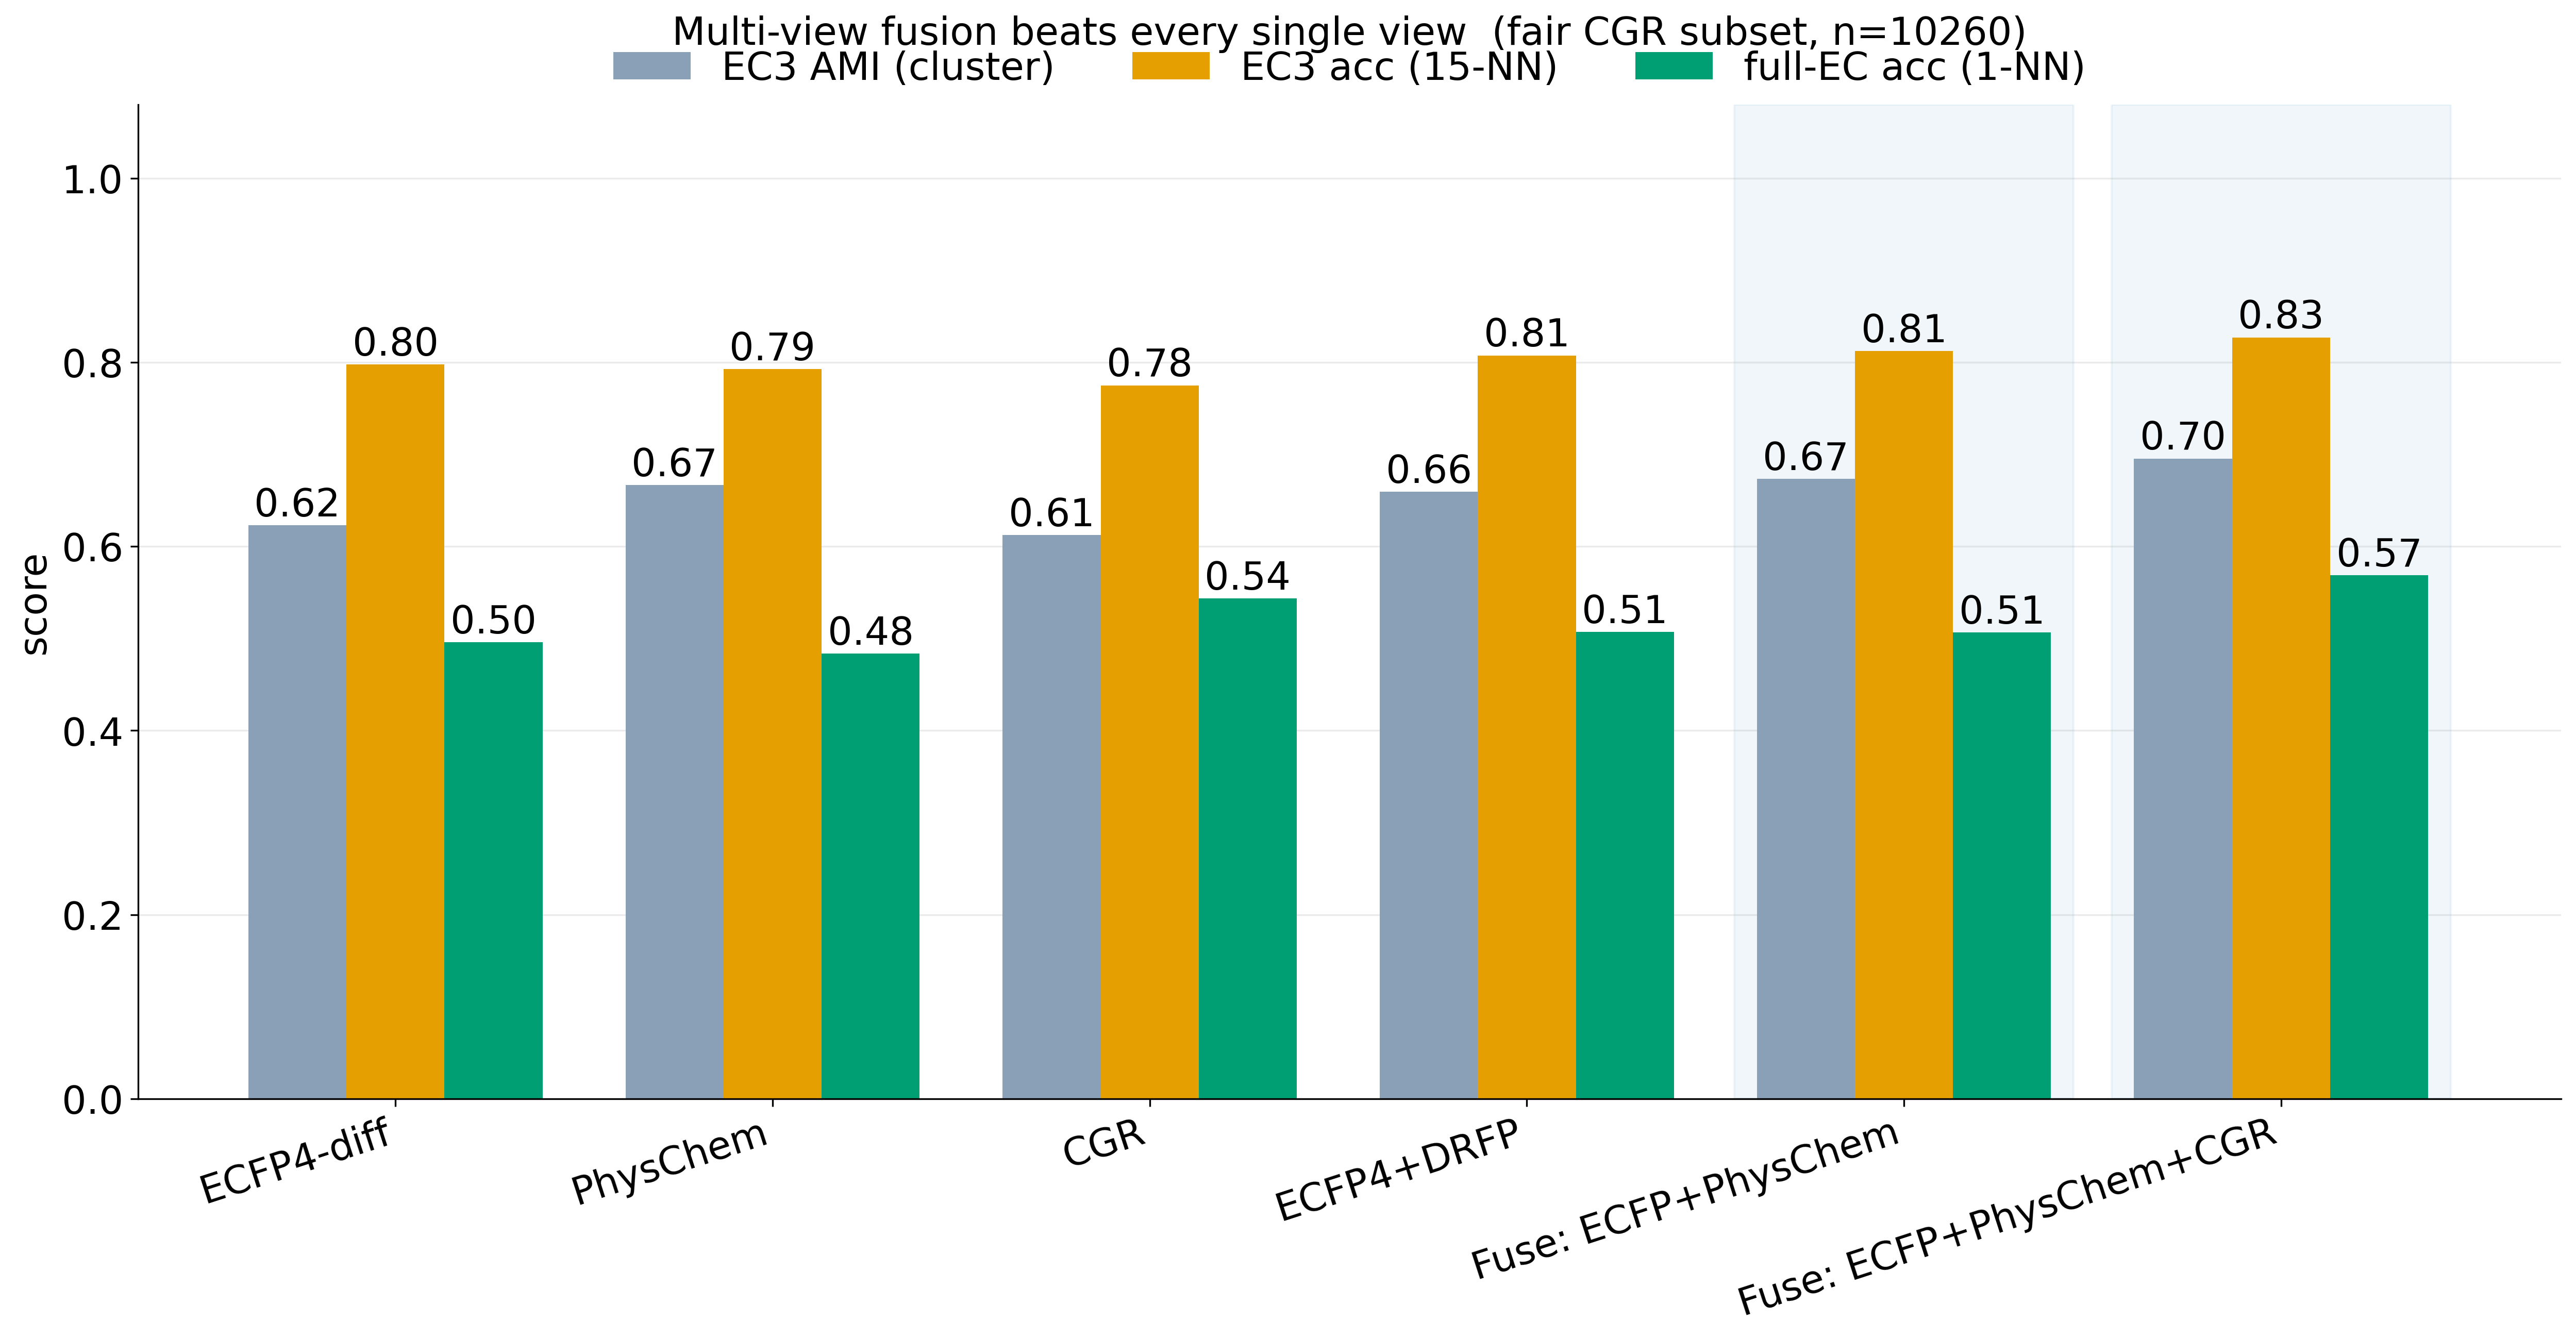
\includegraphics[width=\linewidth]{fig_fusion.png}
    \end{column}
    \begin{column}{0.42\textwidth}\small
      Fuse the complementary views (ECFP $\oplus$ PhysChem $\oplus$ CGR):
      \begin{itemize}
        \item EC3 AMI \best{0.696} --- beats every single view and the best incumbent (0.637).
        \item full-EC 1-NN \best{0.569} --- beats even CGR alone (0.543).
      \end{itemize}
      \textbf{Unsupervised}, no fitting. Each view supplies what the others lack.
      \vspace{4pt}
      \footnotesize Greedy view-selection pushes EC3 AMI to \best{0.718}
      (PhysChem+DRFP core, then diminishing returns) --- gains saturate after $\sim$2 views.
    \end{column}
  \end{columns}
  \takeaway{Fusion of complementary views is a genuine SOTA-beater --- \emph{before} any supervision.}
\end{frame}

% ---------------------------------------------------------------
\begin{frame}{Which combo? --- all 3-view fusions}
  \begin{columns}[T]
    \begin{column}{0.62\textwidth}
      \centering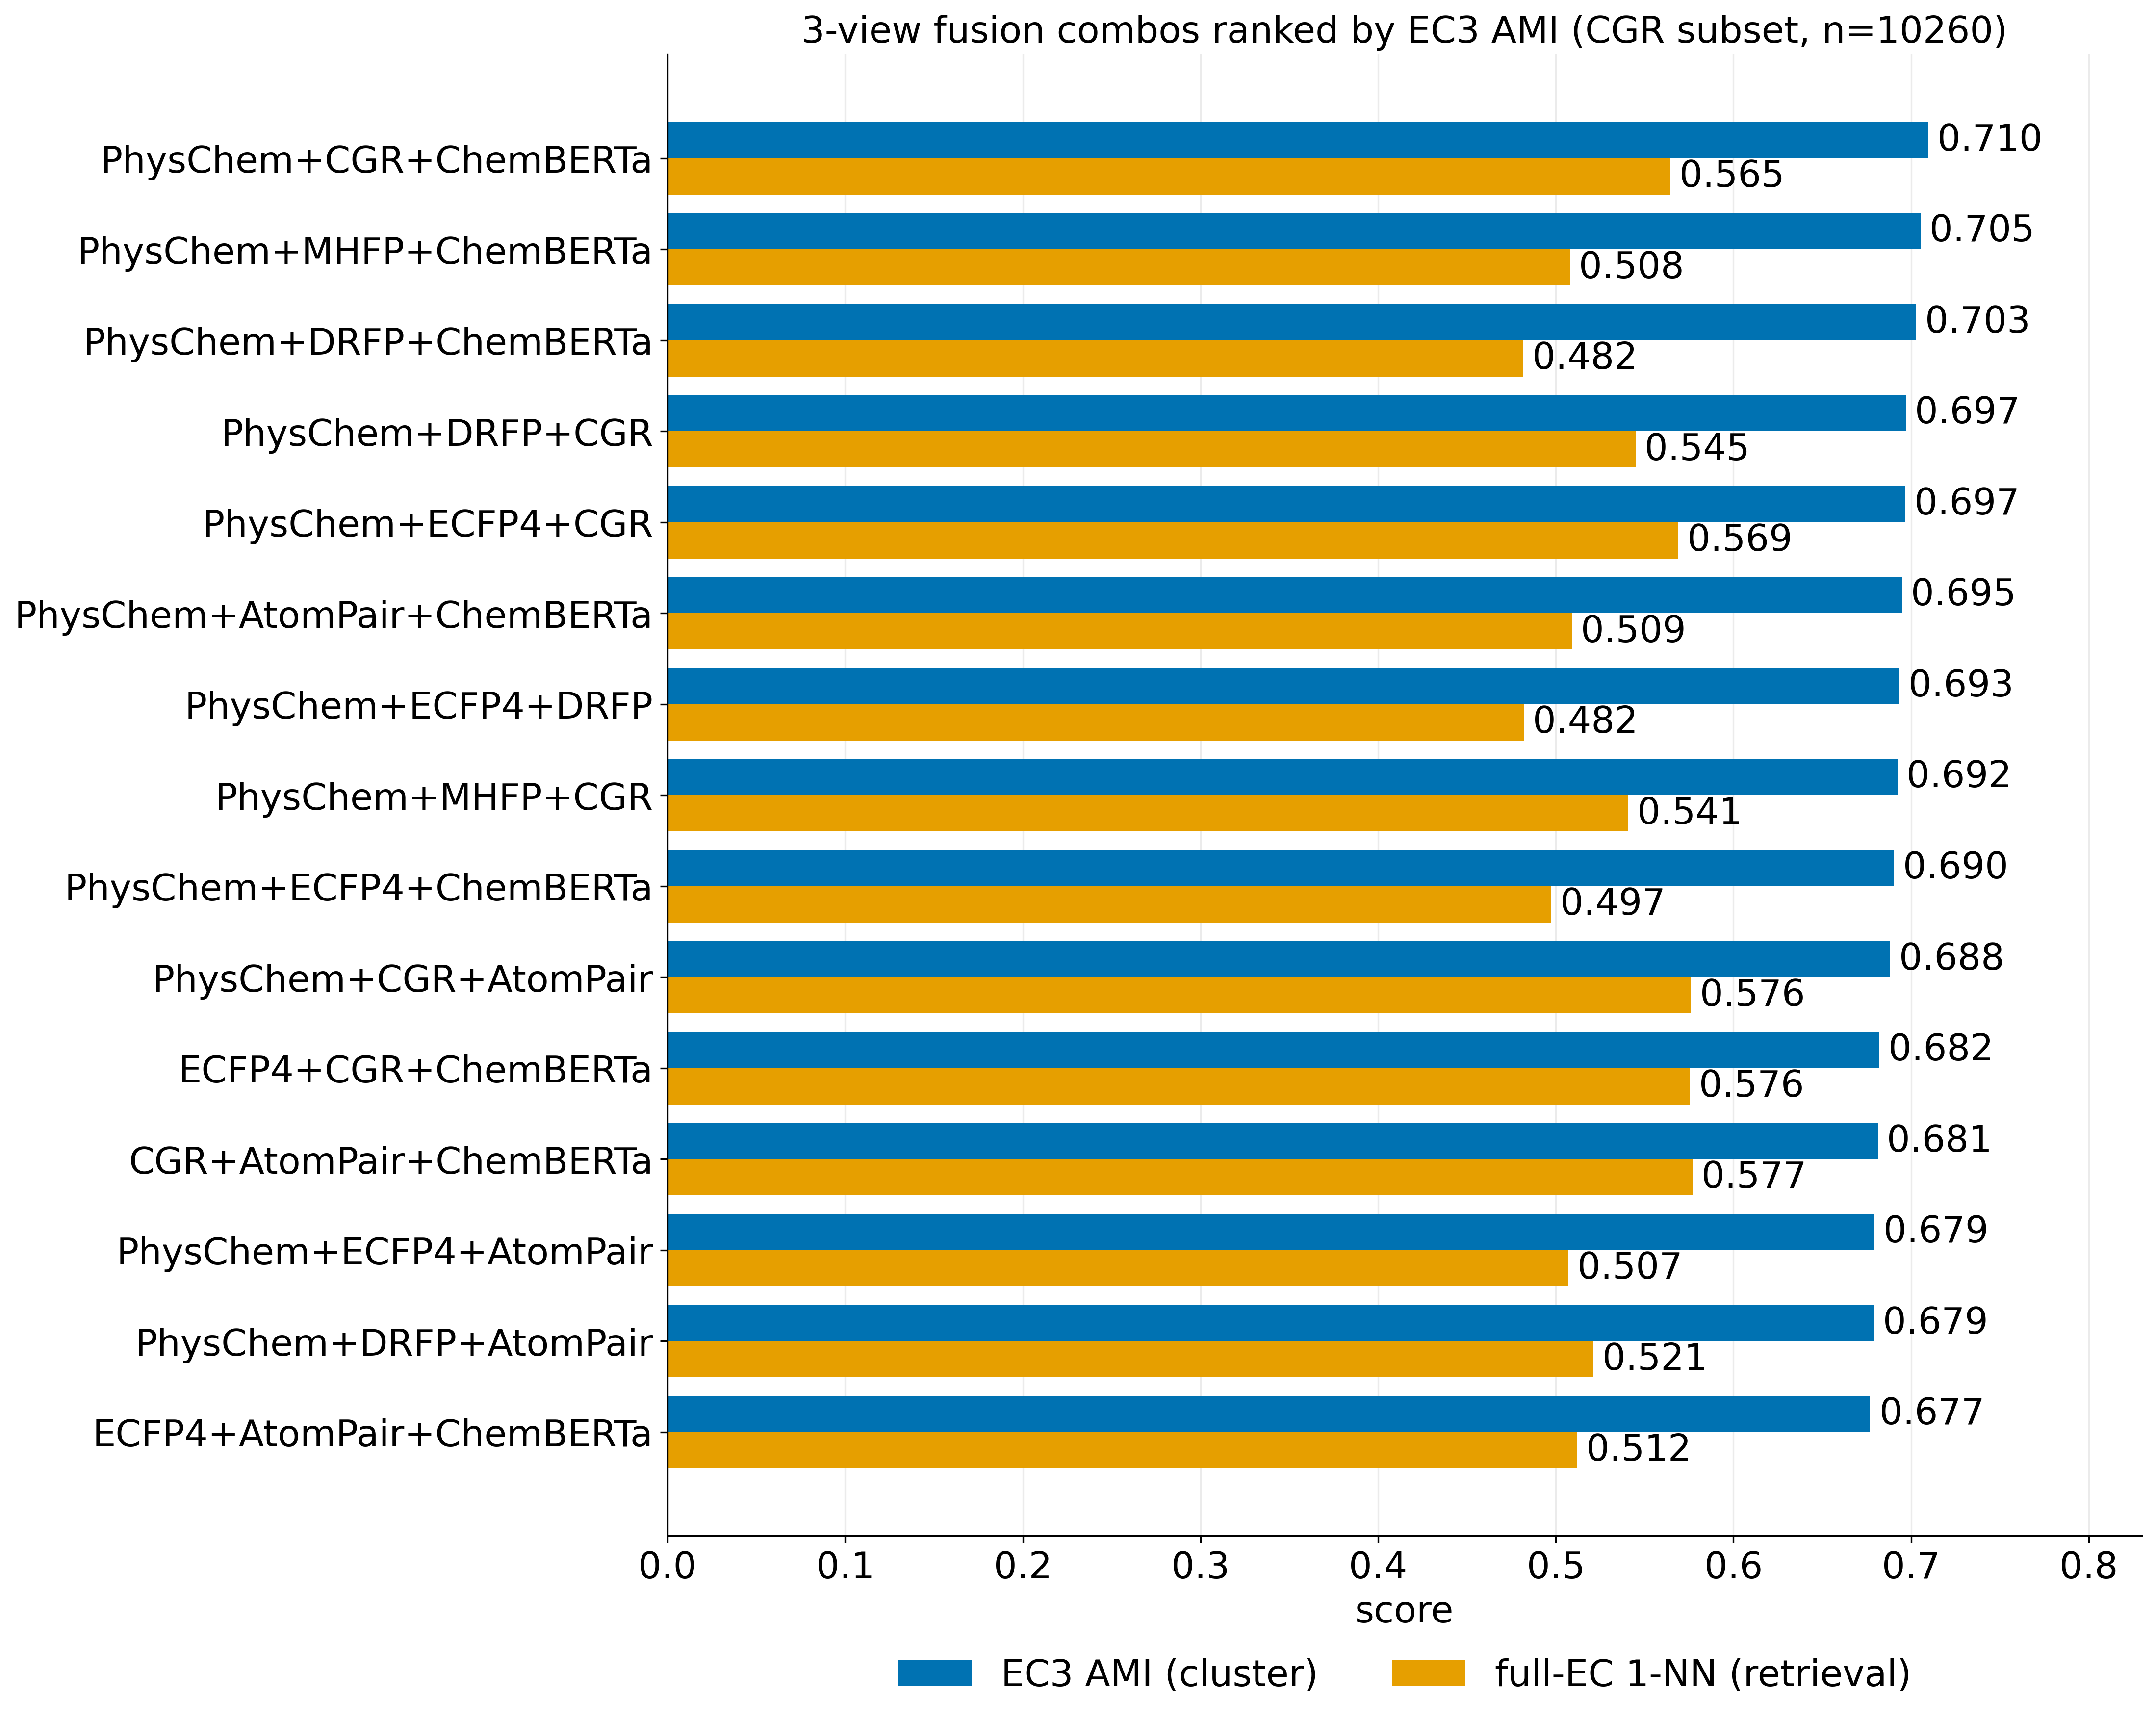
\includegraphics[width=\linewidth]{fig_triple_combos.png}
    \end{column}
    \begin{column}{0.38\textwidth}\small
      All 35 triples from \{\,PhysChem, ECFP4, DRFP, MHFP, CGR, AtomPair, ChemBERTa\,\}
      (PhysChem = 217 physicochemical descriptors).
      \begin{itemize}
        \item \best{PhysChem is the anchor} --- present in every top triple.
        \item Best EC3 AMI: \best{PhysChem+CGR+ChemBERTa (0.71)}.
        \item \best{CGR}-containing triples win \textbf{full-EC retrieval} (0.57--0.58).
        \item Tight band (0.68--0.71): the recipe, not the exact triple, is what matters.
      \end{itemize}
      Even ``weak'' ChemBERTa earns its place in the ensemble.
    \end{column}
  \end{columns}
\end{frame}

% ---------------------------------------------------------------
\begin{frame}{Where this goes --- the ablation ladder}
  \small
  \begin{tabular}{@{}cll@{}}
    \toprule
    Rung & Method & Status / expected\\
    \midrule
    0 & Best incumbent (ECFP/CGR/PhysChem) + agglo & EC3 AMI 0.63--0.67\\
    1 & \textbf{Multi-view fusion} (unsupervised) & \best{0.696 --- done, beats all singles}\\
    2 & + cofactor normalization & de-confound ATP/NAD currency\\
    3 & + self-supervised contrastive & label-free ceiling\\
    4 & + \textbf{hierarchical-EC metric learning} & the label lift (biggest lever)\\
    5 & rung 4, \textbf{held-out EC subclasses} & does it generalize?\\
    \bottomrule
  \end{tabular}
  \vspace{6pt}
  \takeaway{Each rung is one controlled change on the same harness --- so ``beats SOTA'' is decomposable and defensible.}
\end{frame}

% ---------------------------------------------------------------
\begin{frame}{Takeaways}
  \begin{enumerate}\small
    \item \textbf{Structural difference fingerprints + agglomerative-average} are the strong, cheap baseline (EC3 AMI $\approx$0.63); learned reaction embeddings (RXNFP/ChemBERTa/MolFormer) \emph{underperform} them.
    \item \textbf{Retrieval beats clustering} for annotation: confidence-gated 15-NN gives EC3 at 0.90 accuracy over 76\% of reactions.
    \item \textbf{CGR} (atom-mapped bond changes) wins the full-EC retrieval it was designed for, but is coverage-limited and not dominant alone.
    \item \textbf{Multi-view fusion} of complementary views (ECFP $\oplus$ PhysChem $\oplus$ CGR) \best{beats every individual method} --- EC3 AMI 0.70 --- with no supervision.
    \item Next: \textbf{hierarchical-EC metric learning}, evaluated zero-shot on held-out EC subclasses.
  \end{enumerate}
\end{frame}

\end{document}
